\documentclass[12pt, ]{article}

%\usepackage[top=1.5cm,bottom=1cm,left=2cm,right=2cm,a4paper]{geometry}
\usepackage{multirow}
\usepackage{url}
\usepackage{graphicx}
\usepackage{booktabs}
%\graphicspath{{path/}}

\title{Identification of Mutated Genes in Liver Cancer for Survival Prediction}
\author{Javad Razvian}
\date{Aug 17, 2019}



\begin{document}
\maketitle

\section{Introduction}
Liver cancer is common worldwide, more than 600000 deaths from liver cancer are estimated worldwide each year \cite{bib:FMG}.
This study is a try to answer the first part of the question 2 \cite{bib:rtest}. In this part, we determine the 3 most frequently mutated genes in liver cancer, namely ``TP53'', ``TTN'', and ``CTNNB1''. 
The data for Liver Hepatocellular Carcinoma (LIHC)
 is retrieved from  ``The Cancer Genome Atlas" (TCGA)  with the aid of TCGAbiolinks package in R. 
It contains mutation and clinical data for liver cancer in addition to around 50 other cancers or their variations. 

\section{Method}
We focused on the analysis of LIHC samples. In particular, we used TCGAbiolinks to download some samples with mutation. 
In this task, we have used two main packages, namely ``\texttt{maftools}''\cite{bib:maftools} and ``\texttt{TCGAbiolinks}''\cite{bib:tcga}. 
With the help of the latter we got access to liver cancer data and with use of the former we analyzed the data in order to answer the question. 
There were some subtle issues for combining the \texttt{maf} to the \texttt{clinical} data which is explained in the source code. 
There were four types of data in TCGA, called \texttt{muse}, \texttt{mutect}, \texttt{varscan2}, and \texttt{somaticsniper}.
We used all of them for analyzing phase, but they are almost alike; in the report we just show the results of \texttt{mutect} variant as it 
contains more data compare to three other types. 

\section{Results}
As it is shown in the fig.~\ref{fig:mutatedgenes}, ``\textbf{TP53}'', ``\textbf{TTN}'', and ``\textbf{CTNNB1}'' are the 3 most frequently mutated genes in the liver cancer. 
TP53 is the most frequently mutated gene in cancer\cite{bib:BCSP}, it also true in liver cancer based on our results.

\begin{figure}[!htbp]
\centering
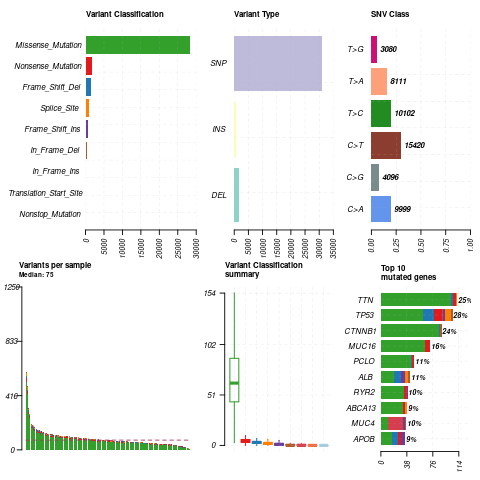
\includegraphics[width=.6\textwidth]{plots/lihc_mutect.png}
\caption{To 10 mutated genes}
\label{fig:mutatedgenes}
\end{figure}


 Which of these genes are more predictive of survival? We can simply answer to this by plotting the Kaplan-Meier survival curve. This plot depicts 
``time to event'' curve. This gives the probability that a patient will survive beyond any specified time. 
In this case study, event is the patient's death. The fig.~\ref{fig:kmplot} shows the KM plot for all of 3 most frequent mutated genes in Liver Cancer. 

\begin{table}[!htbp]
\centering
\begin{tabular}{c|c|c}
    genes  & P-value & Hazard Ratio \\ \midrule
    TTN & 0.837\phantom{00} & 1.08 \\
    CTNNB1 & 0.877\phantom{00} & 1.06 \\
    TP53 & 0.00672 & 2.31 \\
\end{tabular}
\caption{P-values and Hazard Ratio based on KM Plot}
\label{tab:kmplot}
\end{table}

The results of fig.~\ref{fig:kmplot} are summarized in table~\ref{tab:kmplot}. It is obvious that ``TTN'' and ``CTNNB1'' are more predictive to survive. 
As plots show their Mutant genes versus Wild Type genes are very similar and the P-values
also support this fact that these genes have no significant differences with their WTs.
As we know P-value < 0.05 was considered statistically significant.
However the KM plot for ``TP53'' shows that this gene has a great 
effect on patient's death and its P-value (0.00672) confirms this. 

\begin{figure}[!htbp]
\centering
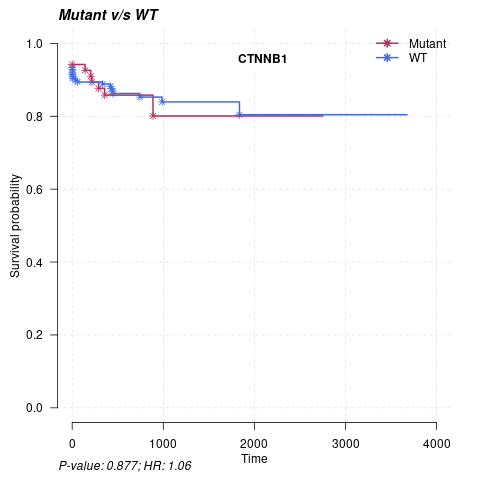
\includegraphics[width=.45\textwidth]{plots/KM_lihc_mutect[CTNNB1].png}
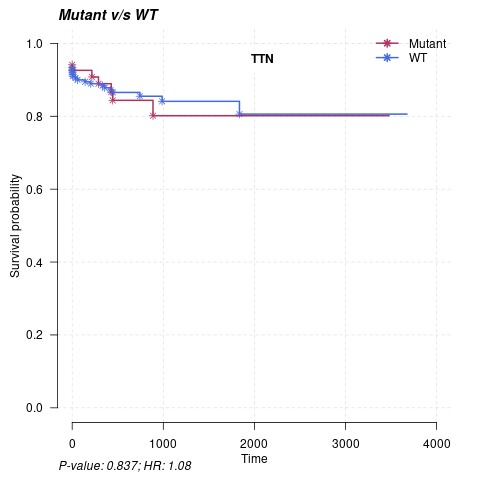
\includegraphics[width=.45\textwidth]{plots/KM_lihc_mutect[TTN].png}
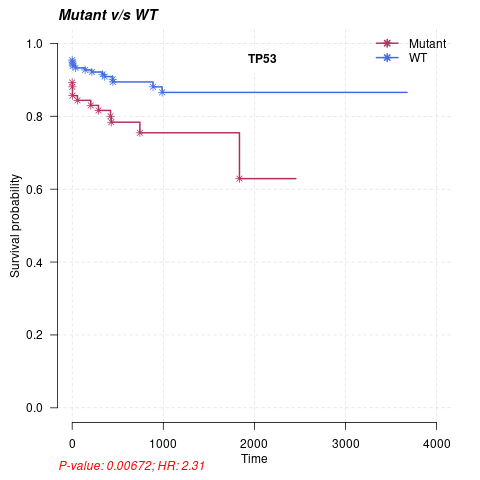
\includegraphics[width=.45\textwidth]{plots/KM_lihc_mutect[TP53].png}
\caption{Kaplan-Meier Curve for Survival Analysis}
\label{fig:kmplot}
\end{figure}


\begin{thebibliography}{9}
    \bibitem{bib:BCSP} Ungerleider, N. A., Rao, S. G., Shahbandi, A., Yee, D., Niu, T., Frey, W. D., \& Jackson, J. G. (2018). Breast cancer survival predicted by TP53 mutation status differs markedly depending on treatment. Breast Cancer Research, 20(1), 115.
    \bibitem {bib:tcga} TCGAbiolinks: An R/Bioconductor package for integrative analysis with GDC data. Available at \url{https://bioconductor.org/packages/release/bioc/html/TCGAbiolinks.html}
    \bibitem {bib:maftools} Summarize, Analyze and Visualize MAF Files. Available at \url{https://bioconductor.org/packages/release/bioc/html/maftools.html}
    \bibitem {bib:rtest}  An R Test. Available at \url{http://oncinfo.org/r_test}.
    \bibitem {bib:FMG} Rao, C. V., Asch, A. S., & Yamada, H. Y. (2016). Frequently mutated genes/pathways and genomic instability as prevention targets in liver cancer. Carcinogenesis, 38(1), 2-11.
    \bibitem {}  Kaplan Meier curve and hazard ratio tutorial, Available at \url{https://www.youtube.com/watch?v=pxRCpcRupgU}.
    \bibitem {} Pancanology Explains Kaplan-Meier Graphs, Available at \url{https://www.youtube.com/watch?v=KE1tkZmWhqU}.


%    \bibitem {}
\end{thebibliography}
\end{document}
